% Generated by LitigCharts.PublicationFigures. Captions and provenance are sidecars.
\documentclass[10pt,tikz,border=5pt]{standalone}
\usepackage{lmodern}
\usetikzlibrary{patterns,patterns.meta}
\begin{document}
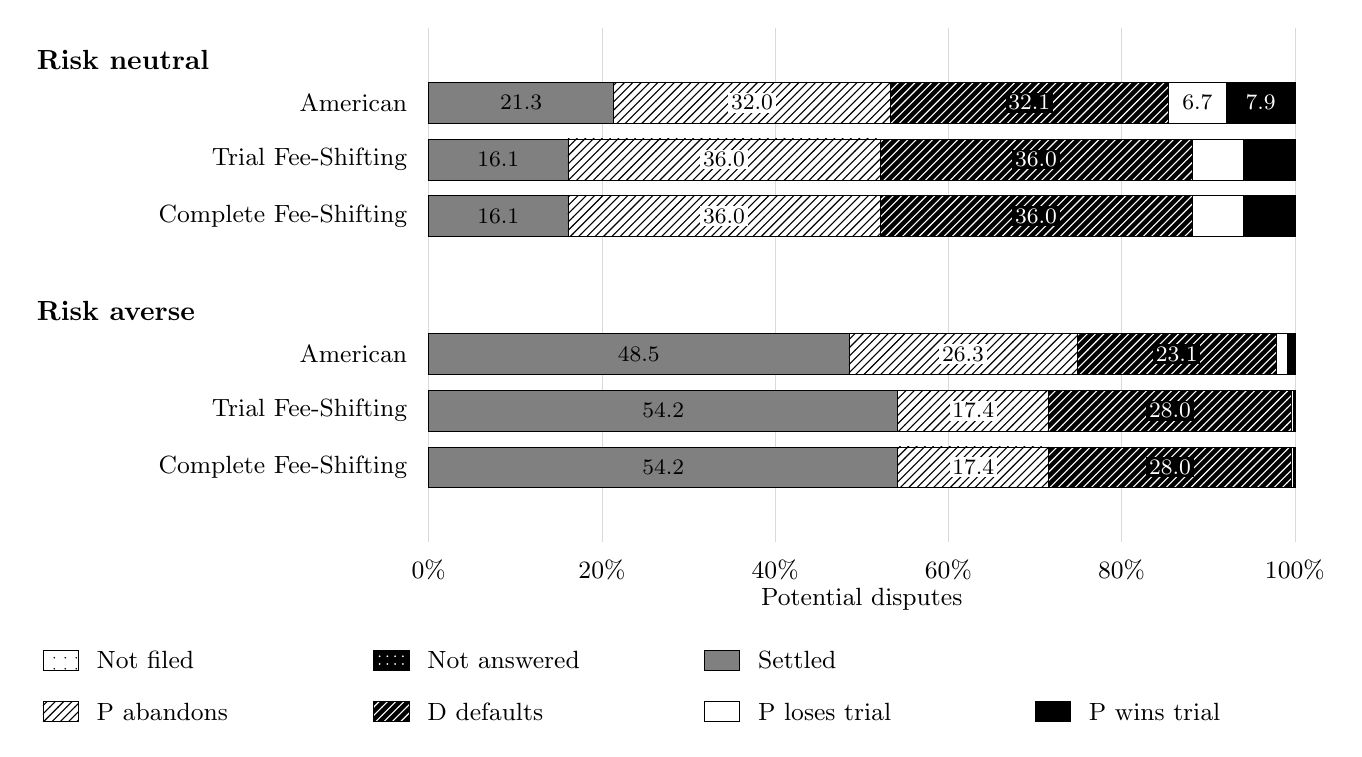
\begin{tikzpicture}[font=\small]\draw[black!15,line width=.2pt] (5.1,.65) -- (5.1,7.18);
\node[anchor=north] at (5.1,.55) {0\%};
\draw[black!15,line width=.2pt] (7.3,.65) -- (7.3,7.18);
\node[anchor=north] at (7.3,.55) {20\%};
\draw[black!15,line width=.2pt] (9.5,.65) -- (9.5,7.18);
\node[anchor=north] at (9.5,.55) {40\%};
\draw[black!15,line width=.2pt] (11.7,.65) -- (11.7,7.18);
\node[anchor=north] at (11.7,.55) {60\%};
\draw[black!15,line width=.2pt] (13.9,.65) -- (13.9,7.18);
\node[anchor=north] at (13.9,.55) {80\%};
\draw[black!15,line width=.2pt] (16.1,.65) -- (16.1,7.18);
\node[anchor=north] at (16.1,.55) {100\%};
\node[anchor=west,font=\bfseries] at (0,6.78) {\mbox{Risk} \mbox{neutral}};
\node[anchor=east] at (4.95,6.23) {American};
\path[fill=black!50,draw=black,line width=.25pt] (5.1,5.97) rectangle (7.447928,6.49);
\node[text=black,fill=none,font=\footnotesize,inner sep=1pt] at (6.273964,6.23) {21.3};
\path[preaction={fill=white,draw=none},pattern={north east lines},pattern color=black,draw=black,line width=.25pt] (7.447928,5.97) rectangle (10.962999,6.49);
\node[text=black,fill=white,font=\footnotesize,inner sep=1pt] at (9.205463,6.23) {32.0};
\path[preaction={fill=black,draw=none},pattern={north east lines},pattern color=white,draw=black,line width=.25pt] (10.962999,5.97) rectangle (14.491974,6.49);
\node[text=white,fill=black,font=\footnotesize,inner sep=1pt] at (12.727486,6.23) {32.1};
\path[fill=white,draw=black,line width=.25pt] (14.491974,5.97) rectangle (15.231105,6.49);
\node[text=black,fill=none,font=\footnotesize,inner sep=1pt] at (14.861539,6.23) {6.7};
\path[fill=black,draw=black,line width=.25pt] (15.231105,5.97) rectangle (16.1,6.49);
\node[text=white,fill=none,font=\footnotesize,inner sep=1pt] at (15.665552,6.23) {7.9};
\node[anchor=east] at (4.95,5.51) {Trial Fee-Shifting};
\path[fill=black!50,draw=black,line width=.25pt] (5.1,5.25) rectangle (6.868679,5.77);
\node[text=black,fill=none,font=\footnotesize,inner sep=1pt] at (5.98434,5.51) {16.1};
\path[preaction={fill=white,draw=none},pattern={north east lines},pattern color=black,draw=black,line width=.25pt] (6.868679,5.25) rectangle (10.831358,5.77);
\node[text=black,fill=white,font=\footnotesize,inner sep=1pt] at (8.850018,5.51) {36.0};
\path[preaction={fill=black,draw=none},pattern={north east lines},pattern color=white,draw=black,line width=.25pt] (10.831358,5.25) rectangle (14.793882,5.77);
\node[text=white,fill=black,font=\footnotesize,inner sep=1pt] at (12.81262,5.51) {36.0};
\path[fill=white,draw=black,line width=.25pt] (14.793882,5.25) rectangle (15.446947,5.77);
\path[fill=black,draw=black,line width=.25pt] (15.446947,5.25) rectangle (16.100001,5.77);
\node[anchor=east] at (4.95,4.79) {Complete Fee-Shifting};
\path[fill=black!50,draw=black,line width=.25pt] (5.1,4.53) rectangle (6.868679,5.05);
\node[text=black,fill=none,font=\footnotesize,inner sep=1pt] at (5.98434,4.79) {16.1};
\path[preaction={fill=white,draw=none},pattern={north east lines},pattern color=black,draw=black,line width=.25pt] (6.868679,4.53) rectangle (10.831358,5.05);
\node[text=black,fill=white,font=\footnotesize,inner sep=1pt] at (8.850018,4.79) {36.0};
\path[preaction={fill=black,draw=none},pattern={north east lines},pattern color=white,draw=black,line width=.25pt] (10.831358,4.53) rectangle (14.793882,5.05);
\node[text=white,fill=black,font=\footnotesize,inner sep=1pt] at (12.81262,4.79) {36.0};
\path[fill=white,draw=black,line width=.25pt] (14.793882,4.53) rectangle (15.446947,5.05);
\path[fill=black,draw=black,line width=.25pt] (15.446947,4.53) rectangle (16.100001,5.05);
\node[anchor=west,font=\bfseries] at (0,3.59) {\mbox{Risk} \mbox{averse}};
\node[anchor=east] at (4.95,3.04) {American};
\path[fill=black!50,draw=black,line width=.25pt] (5.1,2.78) rectangle (10.436573,3.3);
\node[text=black,fill=none,font=\footnotesize,inner sep=1pt] at (7.768287,3.04) {48.5};
\path[preaction={fill=white,draw=none},pattern={north east lines},pattern color=black,draw=black,line width=.25pt] (10.436573,2.78) rectangle (13.333027,3.3);
\node[text=black,fill=white,font=\footnotesize,inner sep=1pt] at (11.8848,3.04) {26.3};
\path[preaction={fill=black,draw=none},pattern={north east lines},pattern color=white,draw=black,line width=.25pt] (13.333027,2.78) rectangle (15.869055,3.3);
\node[text=white,fill=black,font=\footnotesize,inner sep=1pt] at (14.601041,3.04) {23.1};
\path[fill=white,draw=black,line width=.25pt] (15.869055,2.78) rectangle (16.002037,3.3);
\path[fill=black,draw=black,line width=.25pt] (16.002037,2.78) rectangle (16.100006,3.3);
\node[anchor=east] at (4.95,2.32) {Trial Fee-Shifting};
\path[fill=black!50,draw=black,line width=.25pt] (5.1,2.06) rectangle (11.057391,2.58);
\node[text=black,fill=none,font=\footnotesize,inner sep=1pt] at (8.078696,2.32) {54.2};
\path[preaction={fill=white,draw=none},pattern={north east lines},pattern color=black,draw=black,line width=.25pt] (11.057391,2.06) rectangle (12.97281,2.58);
\node[text=black,fill=white,font=\footnotesize,inner sep=1pt] at (12.015101,2.32) {17.4};
\path[preaction={fill=black,draw=none},pattern={north east lines},pattern color=white,draw=black,line width=.25pt] (12.97281,2.06) rectangle (16.056,2.58);
\node[text=white,fill=black,font=\footnotesize,inner sep=1pt] at (14.514405,2.32) {28.0};
\path[fill=white,draw=black,line width=.25pt] (16.056,2.06) rectangle (16.081211,2.58);
\path[fill=black,draw=black,line width=.25pt] (16.081211,2.06) rectangle (16.099994,2.58);
\node[anchor=east] at (4.95,1.6) {Complete Fee-Shifting};
\path[fill=black!50,draw=black,line width=.25pt] (5.1,1.34) rectangle (11.057391,1.86);
\node[text=black,fill=none,font=\footnotesize,inner sep=1pt] at (8.078696,1.6) {54.2};
\path[preaction={fill=white,draw=none},pattern={north east lines},pattern color=black,draw=black,line width=.25pt] (11.057391,1.34) rectangle (12.97281,1.86);
\node[text=black,fill=white,font=\footnotesize,inner sep=1pt] at (12.015101,1.6) {17.4};
\path[preaction={fill=black,draw=none},pattern={north east lines},pattern color=white,draw=black,line width=.25pt] (12.97281,1.34) rectangle (16.056,1.86);
\node[text=white,fill=black,font=\footnotesize,inner sep=1pt] at (14.514405,1.6) {28.0};
\path[fill=white,draw=black,line width=.25pt] (16.056,1.34) rectangle (16.081211,1.86);
\path[fill=black,draw=black,line width=.25pt] (16.081211,1.34) rectangle (16.099994,1.86);
\node at (10.6,-.08) {Potential disputes};
\path[preaction={fill=white,draw=none},pattern={Dots[distance=4pt,radius=.35pt]},pattern color=black,draw=black,line width=.25pt] (0.2,-0.98) rectangle (0.65,-0.72);
\node[anchor=west] at (0.76,-0.85) {Not filed};
\path[preaction={fill=black,draw=none},pattern={Dots[distance=2.8pt,radius=.35pt]},pattern color=white,draw=black,line width=.25pt] (4.4,-0.98) rectangle (4.85,-0.72);
\node[anchor=west] at (4.96,-0.85) {Not answered};
\path[fill=black!50,draw=black,line width=.25pt] (8.6,-0.98) rectangle (9.05,-0.72);
\node[anchor=west] at (9.16,-0.85) {Settled};
\path[preaction={fill=white,draw=none},pattern={north east lines},pattern color=black,draw=black,line width=.25pt] (0.2,-1.63) rectangle (0.65,-1.37);
\node[anchor=west] at (0.76,-1.5) {P abandons};
\path[preaction={fill=black,draw=none},pattern={north east lines},pattern color=white,draw=black,line width=.25pt] (4.4,-1.63) rectangle (4.85,-1.37);
\node[anchor=west] at (4.96,-1.5) {D defaults};
\path[fill=white,draw=black,line width=.25pt] (8.6,-1.63) rectangle (9.05,-1.37);
\node[anchor=west] at (9.16,-1.5) {P loses trial};
\path[fill=black,draw=black,line width=.25pt] (12.8,-1.63) rectangle (13.25,-1.37);
\node[anchor=west] at (13.36,-1.5) {P wins trial};
\end{tikzpicture}
\end{document}
